\section{Análisis de los datos}\label{s:analisis}
El primer paso en todo trabajo de ciencia de datos e inteligencia artificial es el análisis de los datos con los que se cuenta para entrenar y probar el modelo. Por ese motivo, antes de explicar el desarrollo del sistema que será entrenado, se lleva a cabo un estudio preliminar que permitirá la concepción de una idea acerca de cómo se distribuyen los datos con los que se va a trabajar. Se comenzará la sección explicando el origen de los datos y cómo, en bruto, se estructuran (véase la sección \ref{ss:enron}). A continuación, dado que es conveniente adaptar el formato original para el propósito del sistema a desarrollar, el corpus debe prepararse y limpiarse adecuadamente con el fin de eliminar problemas como el ruido y las redundancias (léase el apartado \ref{ss:prep}). Una vez finaliza la importante fase de limpieza de los datos, estos se procesarán para extraer las características que puedan ser de interés y almacenarán en un sistema que mejore la eficiencia respecto a la que se tiene con la estructura original de los datos en bruto (consúltese la sección \ref{ss:almacen}). Por último, se realiza un análisis exploratorio de los datos con el que se describirá el corpus de trabajo y gracias al que se podrá extraer cierta información que será de utilidad en el desarrollo de nuestro sistema de generación de lenguaje natural (el análisis exploratorio de los datos se encuentra en el apartado \ref{ss:eda}).

\subsection{Enron corpus}\label{ss:enron}
Para llevar a cabo cualquier trabajo relacionado con la ciencia de datos e inteligencia artificial es necesario contar con un conjunto de datos con el que poder entrenar al modelo desarrollado. Cuando se trata de un estudio relacionado con la generación de lenguaje natural, el conjunto de datos se llama corpus y suele contener ejemplos de documentos reales redactados por humanos similares a los que se desea producir. En concreto, para este trabajo, se ha elegido el corpus conocido como Enron\footnote{\url{http://www-2.cs.cmu.edu/~enron/}}, dado que los correos electrónicos que contiene pertenecieron a la empresa con el mismo nombre. Precisamente se hicieron públicos tras una investigación legal llevada a cabo a esta compañía por parte de la Comisión Federal de Regulación de la Energía\footnote{\url{https://www.ferc.gov/}} de Estados Unidos.

Enron corpus contiene 517.401 correos electrónicos escritos en inglés de 150 usuarios distintos. Además de la ventaja de la gran cantidad de elementos pertenecientes a este dataset, también ha sido elegido por encontrar diversos trabajos sobre este mismo conjunto de e-mails, como el llevado a cabo por \cite{klimt2004introducing}.

Este corpus está organizado en una jerarquía de directorios (uno por cada usuario), en la que dentro de los principales se encuentran las correspondientes carpetas de la cuenta de correo electrónico del usuario en cuestión, como bandeja de entrada, enviados y directorios personalizados. En estas carpetas se encuentran, cada uno en un archivo separado, los distintos correos electrónicos del corpus. Un ejemplo de cómo se presentan los diferentes e-mails viene reflejado en la figura \ref{fig:emailenron}.

\begin{figure}[h]
	\centering%
	\centerline{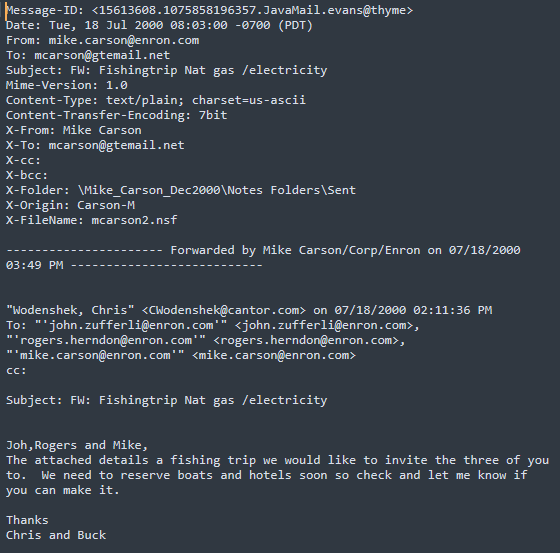
\includegraphics[width = 0.9\textwidth]{Imagenes/Bitmap/email-example.png}}%
	\caption{Ejemplo de un correo electrónico del corpus Enron}%
	\label{fig:emailenron}
\end{figure}

Como puede observarse en la figura \ref{fig:emailenron}, cada uno de los correos electrónicos se encuentra en un archivo distinto estructurado según el formato MIME explicado anteriormente (véase la sección \ref{ss:mime}). Claramente, se pueden diferenciar las distintas cabeceras de este formato con la información correspondiente a cada una de ellas. Después de todas estas cabeceras, se encuentra el cuerpo del mensaje. Por cada uno de los 517.401 correos electrónicos, se encuentra un archivo diferente con esta estructura.

\subsection{Preparación y limpieza de los datos}\label{ss:prep}

El primer problema que aparece ante el conjunto de datos elegidos es el formato en que se presentan cada uno de los correos electrónicos, ya que en cada archivo hay mucha información que generaría ruido y dificultaría el entrenamiento del modelo si no se eliminara (como las cabeceras MIME). Por ese motivo, es necesario preprocesar cada uno de ellos. Asimismo, se conseguiría un dataset apto para el propósito de construir un sistema de generación de lenguaje natural que redacte correos electrónicos.

Para extraer la información relevante de cada uno de ellos, el lenguaje de programación \textit{Python} cuenta con una librería\footnote{\url{https://docs.python.org/3/library/email.parser.html}} capaz de parsear correos electrónicos almacenados en archivos y cadenas de caracteres en formato MIME. Además, una vez procesadas las cadenas, la clase devuelta cuenta con una serie de métodos que facilitan la obtención de la información de las cabeceras y recorrer el árbol de partes MIME (véase la sección \ref{ss:mime} o consúltese el ejemplo de árbol representado en la figura \ref{fig:content-type}). De manera que solo ha sido necesario desarrollar un método que vaya recorriendo la estructura arbórea, comprobando el tipo MIME del nodo, y extrayendo el cuerpo del mensaje cuando lo encuentre.

Una vez se ha resuelto el problema de recuperar el correo electrónico dado el archivo perteneciente al corpus, es posible enfrentarse a otro reto antes del análisis exploratorio de los datos: la limpieza del cuerpo del mensaje para contar con un texto plano de cara al entrenamiento del modelo. Siempre, en todo trabajo en ciencia de datos, se presenta una fase de limpieza de los datos. Este paso resulta ligeramente más complicado cuando se está tratando con cadenas de caracteres. En el caso que ocupa a este trabajo, la limpieza consiste en encontrar patrones externos al cuerpo del mensaje, como la firma o la inclusión del mensaje al que se responde debajo de la respuesta, que no constituyen texto escrito por los usuarios, sino que ha sido incluido por el servidor de correo electrónico. Por ejemplo, en la figura \ref{fig:emailenron}, se muestra un e-mail el cual simplemente está reenviando otro mensaje distinto sin incluir más información. Esto resulta evidente por el comienzo del cuerpo del correo electrónico, que indica el reenvío. Este e-mail no debería incluirse en el entrenamiento de nuestro modelo, porque no añade información nueva y repite un mensaje que ya se tiene en otro archivo (dado que se cuenta con todos los correos del usuario, si el usuario está reenviando un e-mail, significa que es posible encontrar el mensaje original en la bandeja de entrada o alguna de las otras carpetas de su cuenta de correo). Por este motivo, es indispensable limpiar el cuerpo de los todos correos electrónicos del corpus.

Tras analizar concienzudamente el corpus de correos electrónicos se detectan varios patrones que deben abordarse y cambios que tienen que llevarse a cabo en los mensajes. El primero de ellos consiste en que, cuando un usuario contesta a un mensaje, el servidor incluye el mensaje que es respondido debajo de la contestación. En este caso solo interesa la respuesta y no el texto original (pues estará en otro archivo). No obstante, esta casuística no constituye un problema complicado de solventar, ya que se puede distinguir la respuesta del mensaje original porque siempre se incluye una cabecera de texto que no varía. Es decir, basta con encontrar la cabecera como subcadena en el cuerpo y eliminar todo lo que le preceda. La misma solución puede aplicarse al patrón que aparece cuando se envía un correo electrónico modificando una convocatoria de reunión. Resulta que el servidor genera una cabecera para diferenciar la modificación de la convocatoria original.

Ligeramente más complicado respecto a los patrones anteriores, aunque no demasiado, resulta el caso que se muestra en la figura \ref{fig:emailenron}. Se trata del reenvío de un e-mail. Cuando esto ocurre, la cabecera producida por el servidor no se trata de una subcadena fija, sino que incluye como información variable adicional el nombre del usuario que reenvía el correo, así como la fecha y hora en que se produce dicho reenvío. Aunque la solución sea la misma, eliminar lo que preceda a esta cabecera, no basta con buscar una subcadena que no varía, se requiere la utilización de expresiones regulares \citep{thompson1968programming}. Como la gran mayoría de lenguajes de programación, Python cuenta con un módulo para implementar expresiones regulares\footnote{\url{https://docs.python.org/3/library/re.html}} que ha facilitado enormemente esta tarea y ha hecho posible la limpieza de los mensajes con este patrón.

Otro problema que ha sido necesario abordar es el de la firma de los servidores de correo (frases al final de los mensajes como ``Get your FREE download of MSN Explorer''). Al ser siempre iguales, simplemente ha bastado con detectarlos y eliminar dicha subcadena del cuerpo de los mensajes. La dificultad de este tipo de limpieza de texto en realidad reside en detectar estos patrones, ya que, al tratarse de cadenas de caracteres, es complicado detectar incongruencias o errores.

Por último, debido al formato establecido por el protocolo MIME (por lo general depende de la codificación especificada para el mensaje), los servidores de correo electrónico incluyen tabulaciones y saltos de línea con una determinada frecuencia entre las palabras del texto, incluso aunque el usuario no los haya introducido. Dado que el salto de línea o la tabulación no es una información que se considere relevante de cara a la generación de texto de este modelo, se decide transformar estos caracteres en espacios y, a continuación, aplicar las expresiones regulares para detectar las subcadenas en las que se observe más de un espacio en blanco seguido y sustituirlas por uno solo.

Con esto concluye la limpieza de los cuerpos de los mensajes y la fase de preparación de los datos para adaptar los correos electrónicos a un formato adecuado para el sistema de almacenamiento elegido.

\subsection{Procesado y almacenamiento}\label{ss:almacen}

Como se ha explicado en el apartado \ref{ss:enron}, por defecto el corpus se almacena localmente estructurado en una jerarquía de directorios y contando con un archivo por cada correo electrónico. Sin embargo, esta forma de almacenamiento no resulta la más adecuada debido a que imposibilita cualquier método de búsqueda eficiente (sería necesario, en el peor de los casos, abrir todos los archivos para encontrar, por ejemplo, un e-mail en función del identificador del mensaje) y resulta excesivamente lento cuando se pretende procesar todos los mensajes (requiere recorrer la jerarquía como una estructura de datos arbórea entrando en todos los directorios). Por estas razones, la decisión de cambiar el sistema de almacenamiento es acertado para agilizar tanto la carga del corpus como las distintas operaciones que se pueden querer llevar a cabo sobre el mismo.

Como los elementos del conjunto son textos, es decir, datos no estructurados, un almacenamiento clásico en archivos de extensión \textit{.csv} podría provocar problemas como la elección del separador de los distintos campos, habría que utilizar un caracter que no apareciera en ningún cuerpo de mensaje ni en sus otras propiedades (asunto, identificador, destinatario, emisor, etcétera). Por lo tanto, un sistema relacional no parece que sea la mejor opción de almacenamiento para los correos electrónicos. Ante esta situación, se ha elegido el uso del sistema de base de datos NoSQL MongoDB (léase la sección \ref{ss:mongodb}) alojado en la nube\footnote{\url{www.mongodb.com/cloud}}. La decisión de no implantarlo en un repositorio local se sustenta sobre la ventaja que ofrece la nube de disponibilidad desde cualquier dispositivo, lo cual ha sido de gran ayuda en el proceso de desarrollo del trabajo.

Una vez se ha seleccionado la forma de almacenamiento, queda por determinar las colecciones que se van a crear y los campos de los que dispondrán los documentos. Una colección que es indispensable es la que albergará los correos electrónicos, la cual contará con la siguiente estructura:

\begin{python}
{
	# Identificador del documento mongo
	'_id' : ObjectId,
	# Identificador MIME del mensaje
	'Message-ID' : string,
	# Emisor del mensaje
	'From' : string,
	# Destinatario/s del mensaje
	'To' : string,
	# Asunto del mensaje
	'Subject' : string,
	# Cuerpo del mensaje
	'Body' : string,
	# Numero de palabras del cuerpo del mensaje
	'Number_of_Words' : integer,
	# Numero de Information Items del cuerpo del mensaje
	'Number_of_Inits' : integer
}
\end{python}

A excepción de los dos últimos campos, los demás se pueden extraer directamente mediante el uso de la librería específica de Python para mensajes en formato MIME (como se ha explicado en el apartado \ref{ss:prep}). Para obtener los dos últimos, es necesario procesar el cuerpo del mensaje antes de su almacenamiento en la nube. El primero, el número de palabras que contiene el cuerpo del correo electrónico, es posible hallarlo gracias al uso de spaCy (véase la sección \ref{ss:spacy}), librería que no solo tokeniza el texto, sino que nos permite distinguir entre los tokens que son palabras del resto, como, por ejemplo, signos de puntuación.

El último campo del documento que representa a los correos electrónicos, indica el número de Information Items (véase la sección \ref{ss:resumen}) que pueden extraerse del documento siguiendo la implementación llevada a cabo por \cite{genest2010text}. Estos InIts, que se definen como tuplas sujeto-verbo-objeto, se obtienen gracias a la librería textaCy (consúltese el apartado \ref{ss:textacy}), construida a partir de spaCy. De hecho, las representaciones semánticas abstractas que constituyen los Information Items serán la entrada de nuestro sistema de generación de lenguaje natural, por lo que, para evitar volver a extraerlos (su obtención es una operación computacionalmente costosa), será conveniente almacenarlos como otro documento de MongoDB. Dicha colección poseerá la siguiente estructura:

\begin{python}
	{
		# Identificador del documento mongo
		'_id' : ObjectId,
		# Identificador MIME del mensaje del que se extrajo el InIt
		'Message-ID' : string,
		# Sujeto del InIt
		'Subject' : string,
		# Verbo del InIt
		'Verb' : string,
		# Objeto del InIt
		'Object' : string
	}
\end{python}

Por ejemplo, si en el cuerpo del mensaje aparece la construcción lingüística ``I got change'' (en castellano ``tengo cambios''), se obtendrá el Information Item que se muestra en la figura \ref{fig:initexample}. De esta forma, es posible relacionar fácilmente un correo electrónico con sus InIts y viceversa.

\begin{figure}[h]
	\centering%
	\centerline{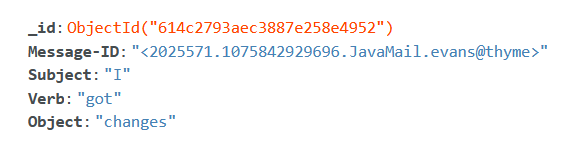
\includegraphics[width = 0.9\textwidth]{Imagenes/Bitmap/initexample.png}}%
	\caption{Ejemplo de documento de un Information Item}%
	\label{fig:initexample}
\end{figure}

Durante el proceso de almacenamiento, también se ha llevado a cabo un primer filtrado de mensajes que no son de utilidad para el propósito que persigue este trabajo y que, por tanto, pueden ser descartados sin guardarlos en MongoDB. Estos son: los correos electrónicos que carecen de cuerpo (puede ser porque originalmente no poseían o porque tras las operaciones de limpieza del mismo que han sido explicadas en la sección \ref{ss:prep}, se produzca esta situación), los e-mails de los que no se extrae ningún Information Item (ya que los InIts serán la entrada de nuestro sistema de generación de lenguaje natural) y los mensajes que son consecuencia de un error en el servidor de mensajería (por ejemplo, al intentar mandar un e-mail con una dirección de destinatario inexistente el servidor de correo siempre manda un mensaje informando de este error). De esta forma, se detectan 35.110 mensajes sin caracteres en el cuerpo, 121.799 correos electrónicos de los que no se extrae ningún Information Item y 7 e-mails consecuencia de errores en el servidor de mensajería, almacenando 360.485 correos electrónicos en la base de datos de MongoDB acompañados de 3.407.099 Information Items.

\subsection{Análisis exploratorio de los datos}\label{ss:eda}
Tras llevar a cabo las tareas de preparación, limpieza de los datos, procesamiento y almacenamiento, con un filtrado a priori, se pueden observar las distribuciones numéricas del corpus desarrollando un análisis exploratorio de los datos. Este estudio preliminar ofrecerá una descripción acerca de los correos electrónicos y sus Information Items.

El primer, y probablemente más sencillo, parámetro que puede analizarse es el número de palabras de cada correo. Para observar cómo se distribuye esta variable en el conjunto de datos, se han calculado las frecuencias requeridas para generar la figura \ref{fig:distpal}. En ella puede deducirse que, a pesar de poseer correos electrónicos con una gigantesca cantidad de palabras, la mayoría de mensajes muestran un número más razonable para tratarse de e-mails.

\begin{figure}[h]
	\centering%
	\centerline{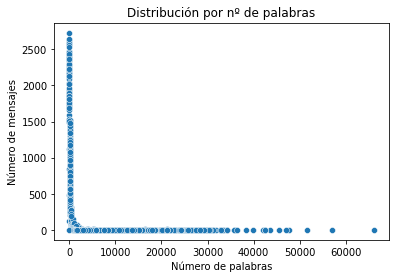
\includegraphics[width = 0.6\textwidth]{Imagenes/Bitmap/dist-palabras.png}}%
	\caption{Distribución del número de palabras en los mensajes}%
	\label{fig:distpal}
\end{figure}

Resulta evidente que la representada en la figura \ref{fig:distpal}, se trata de una distribución con muchos \textit{outliers} por la derecha. En lo que se refiere al apuntamiento, claramente se observa un intervalo relativamente pequeño en el que se concentran una gran cantidad de correos electrónicos. Sin embargo, de dicha gráfica resulta complicado extraer más conclusiones de las mencionadas, por la falta de detalle en la parte más apuntada de la distribución. Por esta razón, se ha delimitado el eje de abscisas y, de esta forma, se puede estudiar en mejores condiciones cómo se distribuye la variable del número de palabras a lo largo del conjunto de datos. El resultado de tomar un intervalo de los primeros valores del eje x (el número de palabras) es la figura \ref{fig:distminpal}.

\begin{figure}[h]
	\centering%
	\centerline{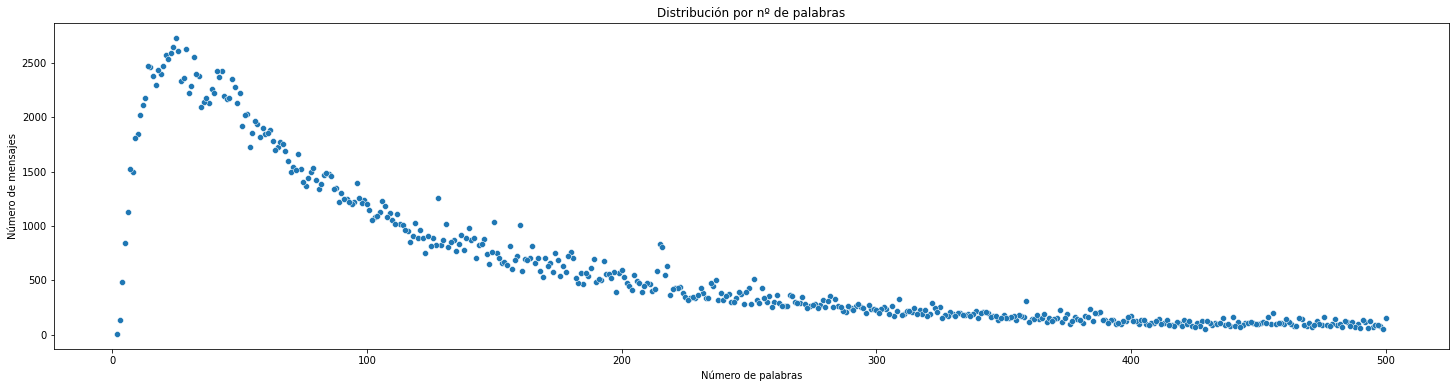
\includegraphics[width = 1.3\textwidth]{Imagenes/Bitmap/dist-mini-palabras.png}}%
	\caption{Distribución del número de palabras en los mensajes delimitando los ejes}%
	\label{fig:distminpal}
\end{figure}

Observando la figura \ref{fig:distminpal}, sí se pueden extraer conclusiones más fundamentadas y con mayor exactitud. Lo más relevante, probablemente sea el hecho de que una amplia cantidad de mensajes del corpus (seguramente un número mayoritario de e-mails) posean menos de doscientas palabras. Esta observación concuerda más con la naturaleza intrínseca del correo electrónico: suelen estar constituidos por un número reducido de oraciones simples y cortas. Resultaría razonable reducir la muestra del corpus en función del número de palabras vista la distribución presentada, pero la decisión del número límite para diferenciar entre los escogidos y los que no resultaría una elección un tanto arbitraria y precipitada si no analizáramos otros parámetros que se ven más adelante. Así que lo más prudente, antes de reducir drásticamente el conjunto de datos en base a un primer vistazo de una variable, es estudiar otras características del corpus.

La otra variable numérica con la que se cuenta en el conjunto de datos es el número de Information Items extraídos del cuerpo del mensaje. Si se analiza la distribución general de esta variable, se obtiene un resultado similar al de la figura \ref{fig:distpal}, pero, como cabe esperar, con valores en el eje de abscisas considerablemente menores (el máximo valor se encuentra cerca de 2500 InIts). Tener menos cantidad de Information Items que de palabras es un resultado coherente con la definición de InIt como tupla sujeto-verbo-objeto. No obstante, la distribución del número de Information Items parece ser, a primera vista, extremadamente más apuntada que la de los mensajes, como queda patente en la figura \ref{fig:distinit}. No obstante, conviene tener en cuenta que aunque siempre se van a extraer menos Information Items que palabras en un correo electrónico, resulta mucho más improbable que dos e-mails coincidan en la cantidad de palabras, la cual varía fácilmente, que en el número de InIts. Esta, es probablemente la causa de que la distribución del número de palabras sea menos apuntada y su curva más suave que la de la cantidad de Information Items.

\begin{figure}[h]
	\centering%
	\centerline{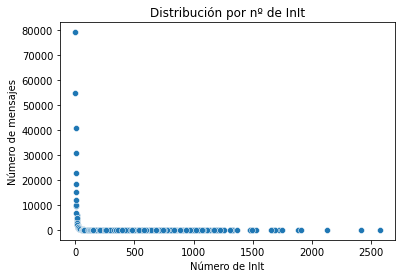
\includegraphics[width = 0.6\textwidth]{Imagenes/Bitmap/distinits.png}}%
	\caption{Distribución del número de Information Items en los mensajes}%
	\label{fig:distinit}
\end{figure}

De nuevo, la figura \ref{fig:distinit}, apenas aporta información detallada acerca de esta variable, por lo que es deseable volver a limitar el eje de abscisas para estudiar el comportamiento de la distribución donde se sitúan la inmensa mayoría de los correos electrónicos del corpus. El resultado de esta restricción del eje x viene dado por la figura \ref{fig:distmininit}, en la cual sí se distinguen fácilmente los distintos valores del eje horizontal y ayuda a sacar conclusiones de la distribución de esta variable.

\begin{figure}[h]
	\centering%
	\centerline{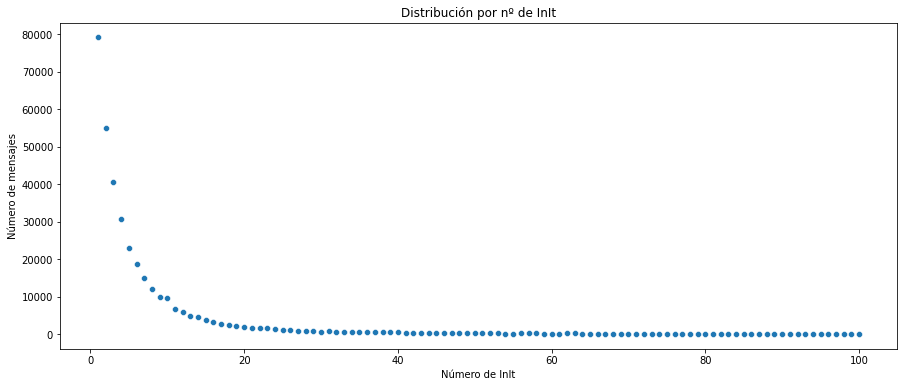
\includegraphics[width = 1.3\textwidth]{Imagenes/Bitmap/distminiinits.png}}%
	\caption{Distribución del número de Information Items en los mensajes delimitando los ejes}%
	\label{fig:distmininit}
\end{figure}

A diferencia de lo que ocurría en la distribución del número de palabras por mensaje, en la que se observaba un crecimiento inicial hasta alcanzar el máximo valor, en el caso de la cantidad de Information Items, la frecuencia de cada valor disminuye gradualmente. Probablemente, esta observación tenga su origen en el hecho de que con un número no tan elevado de InIts, ya se necesite un correo electrónico más largo de lo habitual. Además, existen diferencias sumamente considerables entre las frecuencias de los primeros valores y el resto. Prueba de ello es que se pueden encontrar más de 30.000 correos electrónicos con cuatro Information Items (que si se compara con los 80.000 e-mails con un único InIt también supone una diferencia abismal), mientras que con siete apenas se tienen 15.000 mensajes (ni la mitad).

Antes se comentaba la arbitrariedad que suponía el hecho de reducir el conjunto de datos tomando un límite de número de palabras tan solo habiendo observado las gráficas de su distribución. No obstante, con los Information Items no resulta tan subjetiva esta decisión. Si se conciben los InIts como las entidades informacionales que indican qué se desea tratar en el correo electrónico, resulta razonable pensar que en un e-mail no suelen utilizarse más de cinco o seis Information Items en los casos de mensajes más extensos. Esta percepción viene apoyada por el hecho de que en la distribución los órdenes de magnitud de la frecuencia con la que aparecen los mensajes con muy pocos InIts, son notablemente superiores a la que presentan los correos electrónicos que poseen tres o cuatro Information Items más. Por estos motivos, se plantea la posibilidad de seleccionar aquellos e-mails que no superen un número determinado de InIts. Pero, para elegir este límite se profundizará ligeramente más en la distribución del número de Inits, observando su distribución acumulada normalizada que se muestra en la figura \ref{fig:acuminits}.

\begin{figure}[h]
	\centering%
	\centerline{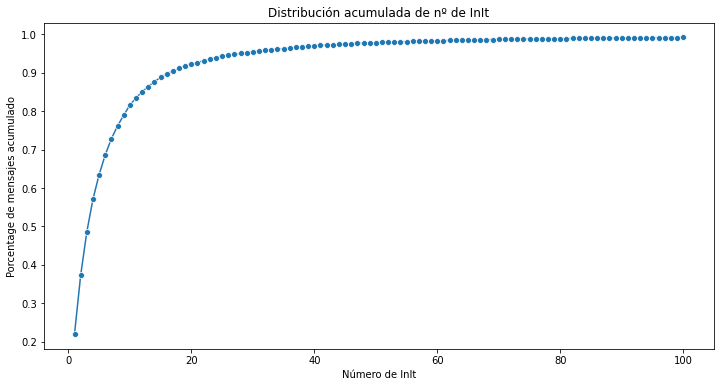
\includegraphics[width = \textwidth]{Imagenes/Bitmap/miniacumporcinit.png}}%
	\caption{Distribución acumulada normalizada del número de Information Items}%
	\label{fig:acuminits}
\end{figure}

La intuición de que un mensaje de gran extensión solía rondar los cinco o seis Information Items, resulta no estar muy distanciada de la realidad ya que, si se observa el valor porcentual correspondiente a la distribución acumulada de una cantidad de seis InIts, se obtendrá una medida cercana al 70\% del total de correos electrónicos del corpus. Concretamente, si se calcula, se obtiene que si se cogieran mensajes con, a lo sumo, seis Information Items, se estaría escogiendo aproximadamente el 68.65\% del corpus almacenado en el sistema de bases de datos, lo que se corresponde con un total de 246.831 correos electrónicos. Esta cantidad suele ser suficientemente grande como para entrenar un modelo de aprendizaje automático satisfactoriamente, por lo que esta reducción de la muestra no solo no afectaría negativamente ni produciría una falta de elementos de entrenamiento, sino que homogeneizaría el conjunto de correos electrónicos de manera que todos tendrían un tamaño razonable acorde a su naturaleza lingüística y versarían sobre un número de temas no excesivamente extenso.

Por todos los motivos expuestos anteriormente, se toma la decisión de llevar a cabo un filtro de mensajes en función de su número de Information Items, teniendo en cuenta aquellos cuya cantidad no supere los seis InIts. A continuación, se entra en detalle acerca de cómo esta reducción ha afectado a la variable del número de palabras en el cuerpo de los mensajes.

\begin{table}[h]
	\begin{tabular}{|l|l|l|l|l|l|l|}
		\hline
		\textbf{Nº de InIts}        & 1     & 2     & 3     & 4      & 5      & 6      \\ \hline
		\textbf{Nº de mensajes}     & 79165 & 54911 & 40628 & 30638  & 22911  & 18578  \\ \hline
		\textbf{Media}              & 43.48 & 70.42 & 95.95 & 118.9  & 138.77 & 176.15 \\ \hline
		\textbf{Desvicación Típica} & 54.15 & 82.43 & 97.89 & 106.17 & 100.21 & 163.81 \\ \hline
		\textbf{Mínimo}             & 2     & 6     & 10    & 14     & 18     & 29     \\ \hline
		\textbf{25\%}               & 16    & 31    & 48    & 65     & 83     & 101    \\ \hline
		\textbf{50\%}               & 29    & 50    & 73    & 94     & 117    & 142    \\ \hline
		\textbf{75\%}               & 51    & 82    & 111   & 138    & 163    & 195    \\ \hline
		\textbf{Máximo}             & 3105  & 4054  & 2647  & 1587   & 2921   & 5218   \\ \hline
		$Q3 + 1.5\cdot RI$ & 103.5  & 158.5  & 205.5  & 247.5   & 283   & 336   \\ \hline
	\end{tabular}
\caption{Estadísticos descriptivos del número de palabras agrupados por el número de Information Items}\label{tab:statswords}
\end{table}

En la tabla \ref{tab:statswords}, se muestran los estadísticos descriptivos de la variable que indica el número de palabras de un mensaje, habiendo agrupado en función del número de Information Items. El detalle que más salta a la vista es el hecho de que, en todos los casos, el valor máximo del conjunto se encuentra siempre muy distante del resto de valores, incluido el tercer cuartil. Esto indica que hay cierto número de outliers en todos los grupos del conjunto de datos. Como esto produce una gran diferencia respecto al resto de mensajes, se considera la posibilidad de eliminarlos de la muestra, razón por la cual se ha incluido como última fila de la tabla el límite superior a partir del cual se definen los outliers o, dicho de otra manera, aquellos elementos que sobrepasen dicho límite se considerarán outliers. Este límite se calcula con la fórmula $Q3 + 1.5\cdot RI$, donde $Q3$ es el tercer cuartil (representado por 75\% en la tabla \ref{tab:statswords}) y $RI$ es el rango intercuartílico, es decir, la diferencia entre el tercer cuartil y el primero.

Como el hecho de eliminar los outliers de estos conjuntos apenas supone una pérdida para el conjunto de datos, se quedaría con 231.288 mensajes de los 246.831, se lleva a cabo esta segunda reducción y se estudia la distribución de la variable de número de palabras en función con la cantidad de Information Items. El resultado de este análisis es la figura \ref{fig:violin}.

\begin{figure}[h]
	\centering%
	\centerline{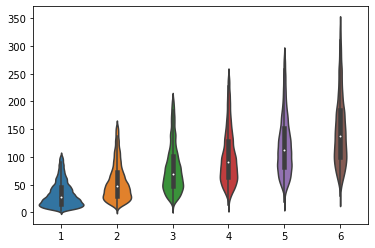
\includegraphics[width = 0.7\textwidth]{Imagenes/Bitmap/violininitword.png}}%
	\caption{Distribución del número de palabras en función del número de Information Items}%
	\label{fig:violin}
\end{figure}

Las distribuciones presentes en la figura \ref{fig:violin}, resultan bastante razonables en cuanto al número de palabras se refiere cuando se habla de correos electrónicos. Todas ellas presentan asimetría positiva y, conforme se aumenta el número de Information Items, el apuntamiento se reduce considerablemente, lo que es consecuencia de que los elementos estén menos concentrados alrededor de la media y la mediana. Conviene también resaltar, que las distribuciones son coherentes con la definición de InIt, ya que conforme aumenta la cantidad de Information Items, la media, mediana y cuartiles del número de palabras aumenta.

Con esta última reducción se cuenta con un conjunto de datos bastante homogéneo y acorde con el tipo de correos electrónicos que se pretende generar: con una longitud razonable no muy extensa (hasta aproximadamente 350 palabras) y con un número de Information Items menor o igual a seis. Resumiendo el análisis exploratorio de datos, inicialmente se ha observado una distribución del número de palabras excesivamente dispersa, al igual que el número de InIts. Para solventar este problema se ha filtrado el conjunto de datos eliminando aquellos mensajes que poseyeran más de seis Information Items. A continuación, estudiando el conjunto resultante, se han quitado los outliers, obteniendo la distribución final representada en la figura \ref{fig:violin}.